\subsection{Производная по направлению}

\begin{tbox}{Базис в пространстве \(\mathbb{R}^k\)}
	Вектора \(\vec{e}_1 = (1,0,\dots, 0)\), \(\vec{e}_2 = (0,1,\dots, 0)\), \(\dots\), \(\vec{e}_k = (0,0,\dots, 1)\) называются \uline{базисом в пространстве \(\mathbb{R}^k\)}. Если \(\vec{x} = (x_1, x_2, \dots, x_k) \in \mathbb{R}^k\), то этот вектор можно разложить по векторам базиса следующим образом:

	\begin{equation*}
		\boxed{
			\vec{x} = x_1 \vec{e}_1 + x_2 \vec{e}_2 + \dots + x_k \vec{e}_k = \sum_{i=1}^k x_i \vec{e}_i
		}
	\end{equation*}

	Для \(\mathbb{R}^3\) часто используются обозначения:
	\[
	\vec{i} = (1,0,0), \quad \vec{j} = (0,1,0), \quad \vec{k} = (0,0,1).
	\]

	Тогда любой вектор \(\vec{a} = (x, y, z) \in \mathbb{R}^3\) можно записать как:
	\[
	\vec{a} = x \vec{i} + y \vec{j} + z \vec{k}.
	\]
\end{tbox}

\begin{tbox}{Производная по направлению}
	Пусть в \(\mathbb{R}^k\) задана функция \(y = f(\vec{x})\), где \(\vec{x} \in E \subset \mathbb{R}^k\) и \(\vec{x}_0 \in E \subset \mathbb{R}^k\). Выберем единичный вектор \(\vec{l} \in \mathbb{R}^k\), задающий направление, причем \(\|\vec{l}\| = 1\).

	Если существует предел:
	\[
	\exists \lim_{t \to 0} \frac{f(\vec{x}_0 + t \cdot \vec{l}) - f(\vec{x}_0)}{t},
	\]
	то его называют \textbf{производной функции \(f(\vec{x})\) в точке \(\vec{x}_0\) по направлению \(\vec{l}\)} и обозначают:
	\begin{equation*}
		\frac{\partial f(\vec{x}_0)}{\partial l} = \lim_{t \to 0} \frac{f(\vec{x}_0 + t \cdot \vec{l}) - f(\vec{x}_0)}{t}.
	\end{equation*}
\end{tbox}

\begin{tbox}{Частная производная}
	Частная производная функции \(f(\vec{x})\) по переменной \(x_i\) определяется как:
	\begin{equation*}
		\frac{\partial f(\vec{x}_0)}{\partial x_i} = \lim_{\Delta x_i \to 0} \frac{\Delta_i f(\vec{x}_0)}{\Delta x_i},
	\end{equation*}
	где
	\[
	\Delta_i f(\vec{x}_0) = f(x_{0_1}, ..., x_{0_{i-1}}, x_{0_i} + \Delta x_i, x_{0_{i+1}}, ..., x_{0_k}) - f(x_{0_1}, ..., x_{0_{i-1}}, x_{0_i}, x_{0_{i+1}}, ..., x_{0_k}).
	\]

	Разложение приращения аргумента по базису:
	\[
	\Delta \vec{x} = (0, \dots, 0, \Delta x_i, 0, \dots, 0) = \Delta x_i \cdot \vec{e}_i.
	\]

	Тогда:
	\begin{equation*}
		\frac{\partial f(\vec{x}_0)}{\partial x_i} = \lim_{\Delta x_i \to 0} \frac{f(\vec{x}_0 + \Delta x_i \cdot \vec{e}_i) - f(\vec{x}_0)}{\Delta x_i}.
	\end{equation*}

	Если обозначить \(\Delta x_i = t\), то:
	\begin{equation*}
		\frac{\partial f(\vec{x}_0)}{\partial x_i} = \lim_{t \to 0} \frac{f(\vec{x}_0 + t \cdot \vec{e}_i) - f(\vec{x}_0)}{t} = \frac{\partial f(\vec{x}_0)}{\partial e_i}.
	\end{equation*}

	Таким образом, \textbf{частная производная по переменной \(x_i\)} — это \textbf{производная по направлению соответствующего базисного вектора \(\vec{e}_i\)}.
\end{tbox}

\begin{tbox}{Производная по направлению для функции двух переменных}
	Рассмотрим функцию \(z = f(x, y)\) и точку \(M_0(x_0, y_0)\):

	\begin{align*}
		\frac{\partial z(M_0)}{\partial x}  = \lim_{\Delta x \to 0} \frac{f(x_0 + \Delta x, y_0) - f(x_0, y_0)}{\Delta x} = \frac{\partial f(M_0)}{\partial i} \quad& \text{(\Cref{fig:2.11.1.1})}\\
		\frac{\partial z(M_0)}{\partial y}  = \lim_{\Delta y \to 0} \frac{f(x_0, y_0 + \Delta y) - f(x_0, y_0)}{\Delta y} = \frac{\partial f(M_0)}{\partial i} \quad& \text{(\Cref{fig:2.11.1.2})}\\
		\frac{\partial z(M_0)}{\partial l} = \lim_{\Delta t \to 0} \frac{f(x_0 + t \cos \alpha, y_0 + t \cos \beta) - f(x_0, y_0)}{t} \quad&\text{(\Cref{fig:2.11.1.3})}
	\end{align*}

	Пусть \(\vec{l} \in \mathbb{R}^2\), \(\|\vec{l}\| = 1\), \(\vec{l} = (\cos \alpha, \cos \beta)\), где:
	\begin{itemize}
		\item \(\alpha\) — угол между вектором \(\vec{l}\) и осью \(Ox\),
		\item \(\beta\) — угол между вектором \(\vec{l}\) и осью \(Oy\).
	\end{itemize}
	\begin{figure}[H]
		\centering
		\begin{minipage}{0.32\linewidth}
			\centering
			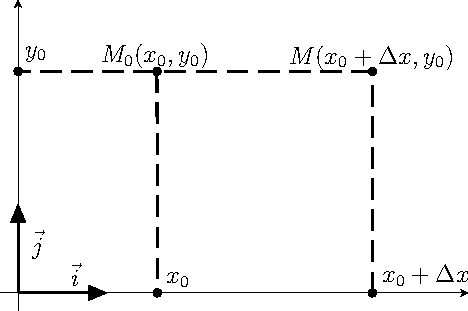
\includegraphics[width=\linewidth]{2.pdf}
			\subcaption{ }
			\label{fig:2.11.1.1}
		\end{minipage}
		\begin{minipage}{0.32\linewidth}
			\centering
			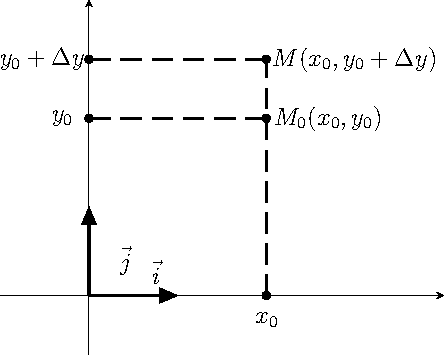
\includegraphics[width=\linewidth]{3.pdf}
			\subcaption{ }
			\label{fig:2.11.1.2}
		\end{minipage}
		\begin{minipage}{0.32\linewidth}
			\centering
			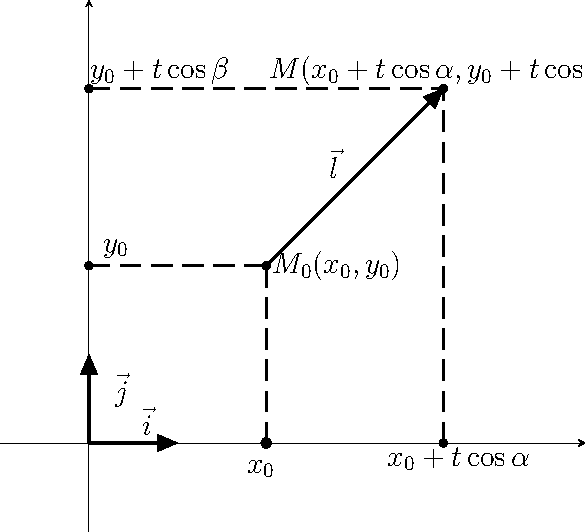
\includegraphics[width=\linewidth]{4.pdf}
			\subcaption{ }
			\label{fig:2.11.1.3}
		\end{minipage}
		\caption{ }
		\label{fig:2.11.1}
	\end{figure}
\end{tbox}

\begin{tbox}{Теорема о связи производной по направлению с градиентом}
	Если функция $y = f(\vec{x})$ дифференцируема в точке $\vec{x}_0 \in E \subset \mathbb{R}^k$, то существуем производная по любому направлению $\vec{l}$, $\vec{l} \in \mathbb{R}^k$, $||\vec{l} = 1||$, и вычисляется это производная по формуле:
	\begin{equation*}
		\frac{\partial f(\vec{x}_0)}{\partial l} = (\grad f(\vec{x}_0), \, l)
	\end{equation*}
	\subsubsection*{Доказательство}

	Так как функция $y = f(\vec{x})$ дифференцируема в точке $\vec{x}_0$, то ее приращения в этой точке можно представить в виде:
	\begin{equation} \label{eq:6.1}
		\Delta f(\vec{x}_0) = f(\vec{x}) - f(\vec{x}_0) = \left(\vec{A}, \, \Delta \vec{x}\right) + \left(\vec{\alpha}(\Delta \vec{x}), \, \Delta \vec{x}\right),
	\end{equation}
	где $\vec{A} = \grad f(\vec{x}_0)$ -- постоянный вектор, координатами этого вектора является частные производные.
	\begin{equation*}
		\begin{aligned}
			\vec{A} = \left(\frac{\partial f(\vec{x}_0)}{\partial x_1}, \, \frac{\partial f(\vec{x}_0)}{\partial x_2}, ..., \frac{\partial f(\vec{x}_0)}{\partial x_k}\right) && \vec{\alpha}(\Delta \vec{x}) \to \vec{\theta} && \Delta \vec{x} \to \vec{\theta}
		\end{aligned}
	\end{equation*}
	Точку представим в виде:
	\begin{align*}
		\vec{x} = \Delta \vec{x} + \vec{x}_0 = \left[\Delta \vec{x} = t \cdot \vec{l}\,\right] = \vec{x}_0 + t \cdot \vec{l} && \Delta \vec{x} \to \vec{0} \text{, при }t \to 0
	\end{align*}

	Подставим в выражение \cref{eq:6.1}:
	\begin{multline*}
		f(\vec{x}_0 + t \cdot \vec{l}) - f(\vec{x}_0) = \left(\grad f(\vec{x}_0), \, t \cdot \vec{l}\,\right) + \left(\vec{\alpha}(t \cdot \vec{l}), \, t \cdot \vec{l}\,\right) = \\= \left(\grad f(\vec{x}_0), \, \vec{l} \,\right) \cdot t + \left(\vec{\alpha}(t \cdot \vec{l}), \, \vec{l}\,\right) \cdot t
	\end{multline*}
	\[\lim_{t \to 0} \frac{f(\vec{x}_0 + t \cdot \vec{l}) - f(\vec{x}_0)}{t} = \lim_{t \to 0} \left[\left(\grad f(\vec{x}_0), \vec{l}\,\right) + \left(\vec{\alpha}(t \cdot \vec{l}), \vec{l}\,\right)\right] = \left(\grad d \, f(\vec{x}_0), \vec{l}\,\right)\]
\end{tbox}

\subsubsection*{Пример}
Дана функция:
\[ u = xy - z^2 \]

Требуется найти производную этой функции в направлении биссектрисы первого координатного угла \( xoy \) в точке \( M_0(-9, 12, 10) \).

\vspace{0.5em}
\begin{enumerate}
	\item \textbf{Вычисление градиента функции \( u \):}
	\[
	\grad u = \left( \frac{\partial u}{\partial x}, \frac{\partial u}{\partial y}, \frac{\partial u}{\partial z} \right) = y \cdot \vec{i} + x \cdot \vec{j} - 2z \cdot \vec{k}
	\]
	В точке \( M_0 \):
	\[
	\grad u(M_0) = 12 \vec{i} - 9 \vec{j} - 20 \vec{k}
	\]
	\item \textbf{Направление биссектрисы \( xoy \):}\\
	Биссектриса первого координатного угла имеет направляющие косинусы:
	\[
	\cos \alpha = \frac{1}{\sqrt{2}}, \quad \cos \beta = \frac{1}{\sqrt{2}}, \quad \cos \gamma = 0
	\]
	Таким образом, вектор направления:
	\[
	\vec{l} = \left(\cos \alpha, \cos \beta, \cos \gamma\right) = \frac{1}{\sqrt{2}} \vec{i} + \frac{1}{\sqrt{2}} \vec{j}
	\]
	\item \textbf{Производная в направлении \( \vec{l} \):}
	\[
	\frac{\partial u(M_0)}{\partial l} = \left( \grad u(M_0), \vec{l} \,\right) = 12 \cdot \frac{1}{\sqrt{2}} + (-9) \cdot \frac{1}{\sqrt{2}} = \frac{3}{\sqrt{2}}
	\]

	\textbf{Итоговый ответ:}
	\[
	\frac{\partial u(M_0)}{\partial l} = \frac{3}{\sqrt{2}}
	\]
\end{enumerate}
%\begin{figure}[H]
%	\centering
%	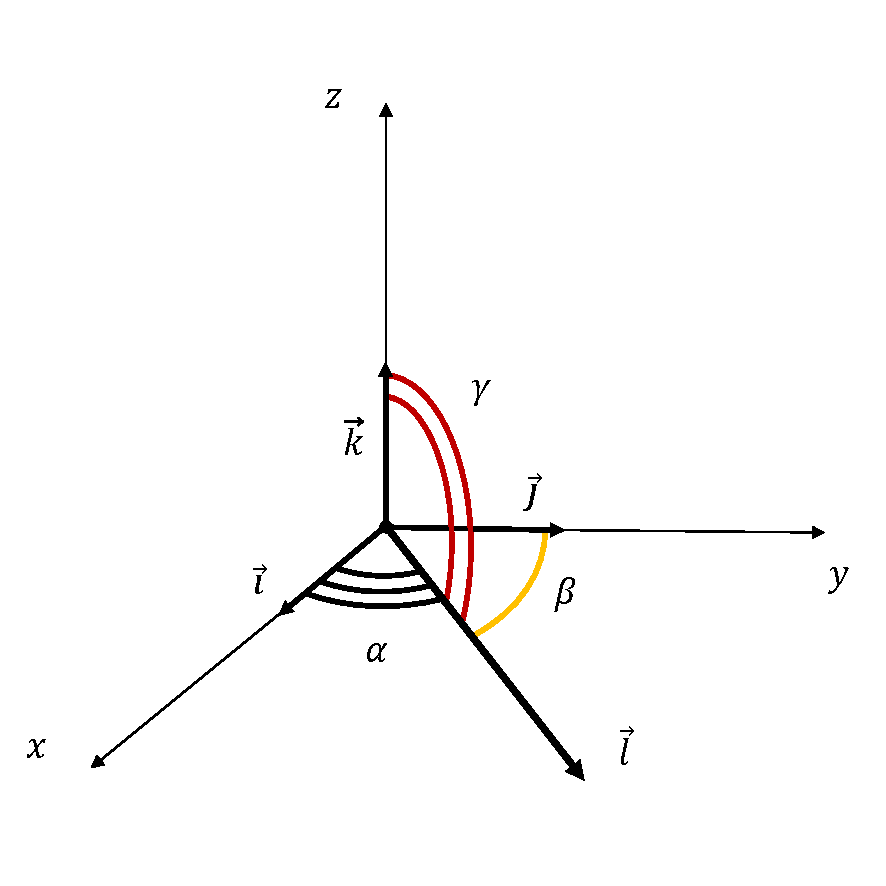
\includegraphics[width=0.5\linewidth]{5.pdf} % Укажите высоту, если нужно
%	\caption{ }
%	\label{fig:18}
%\end{figure}